\section{Fourier-Transformation}{120}

Im Gegensatz zu den Fourier-Reihen, welche ausschliesslich periodische Signale 'verarbeiten' können, beschäftigt sich die 
Fourier-Transformation mit \textbf{nicht-periodischen Signalen!}


\subsection{Existenz des Fourier-Integrals}{131}

Die Fourier-Transformation von $f(t)$ und die inverse Fourier-Transformation existieren, wenn:

\subsubsection{Bedingung 1}

\vspace{-0.2cm}

$$ \boxed{ \int\limits_{- \infty}^{\infty} | f(t) | \, \diff t < \infty  \quad \text{ \textrightarrow\ \textbf{$\bm{f(t)}$ ist absolut integrierbar} }} $$

Diese Bedingung ist \textbf{hinreichend}, aber \textbf{nicht notwendig}!


\subsubsection{Bedingung 2}

$f(t)$ ist fouriertransformierbar, wenn:
$$ \boxed{ \int\limits_{- \infty}^{\infty} | F(\jimg \omega) | \, \diff \omega < \infty } $$

\textrightarrow\ \textbf{Die Fourier-Transformation $F(\jimg \omega)$ ist absolut integrierbar} 


\subsubsection{Bedingung 3}

$f(t)$ ist fouriertransformierbar, wenn:
\vspace{0.2cm}

\textbf{$\bm{f(t)}$ eine Linearkombination absolut integrierbarer Funktionen $\bm{f_i(t)}$ und inverser Fourier-Transformationen 
von $\bm{F_i(\jimg \omega)}$, die selber absolut integrierbar sind, ist.} 


\subsection{Berechnung der Fouriertransformation}{121}

\vspace{-0.2cm}	

$$ \boxed{ \text{Fouriertransformierte: \quad} F(\jimg \omega) = \int \limits_{-\infty}^{\infty} f(t) \, \e^{- \jimg \omega t} \, \diff t  } $$
$$ \boxed{ \text{Rücktransformation: \quad} f(t) = \frac{1}{2 \pi} \int \limits_{-\infty}^{\infty} F(\jimg \omega) \, \e^{\jimg \omega t} \, \diff \omega } $$		
		
$F(\jimg \omega)$ wird Fouriertransformierte oder \textbf{Spektralfunktion} genannt	


\subsubsection{Tipp: Berechnung von $\bm{F(0)}$}

\vspace{-0.2cm}	

$$ \boxed{ F(0) = \int \limits_{-\infty}^{\infty} f(t) \, \e^{- \jimg 0 t} \, \diff t =  \int \limits_{-\infty}^{\infty} f(t) \, \diff t } $$


\subsection{Konvergenzgeschwindigkeit}{122-123}

Je glatter eine Zeitfunktion $f(t)$ ist, desto schneller fällt ihre Fourier-Transformierte $F(\jimg \omega)$ ab und umgekehrt

% Idee: links und rechts von Hand Zeichnungen aus Vorlesungen dazumachen

\begin{center}
	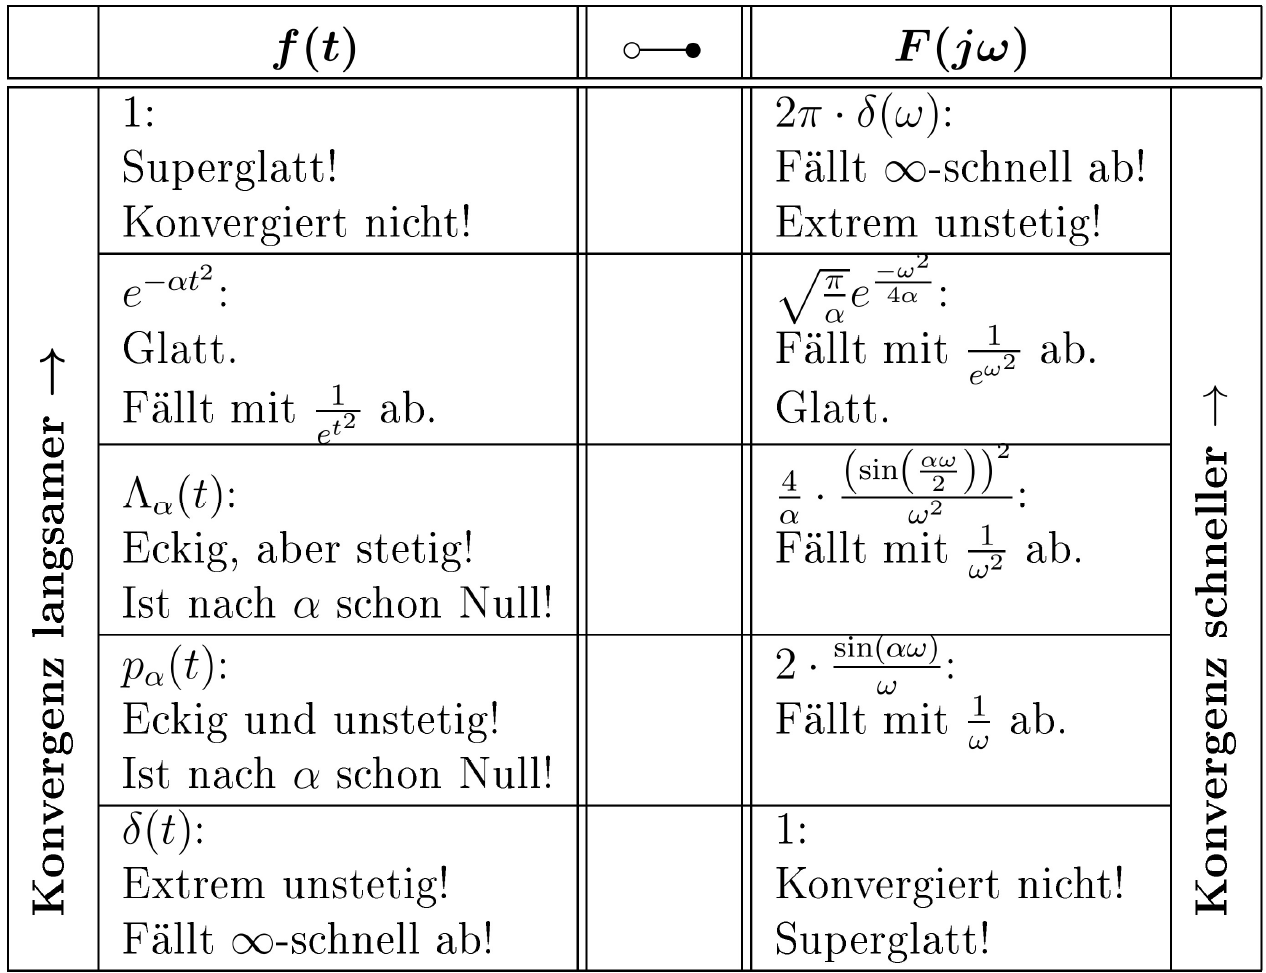
\includegraphics[width=0.7\columnwidth]{images/konvergenzgeschwindigkeit.png}
\end{center}

Im Frequenzbereich passiert das \textbf{duale} zum Zeitbereich!


\subsection{Eigenschaften der Fourier-Transformation}{124-130}

\subsubsection{Übersicht}

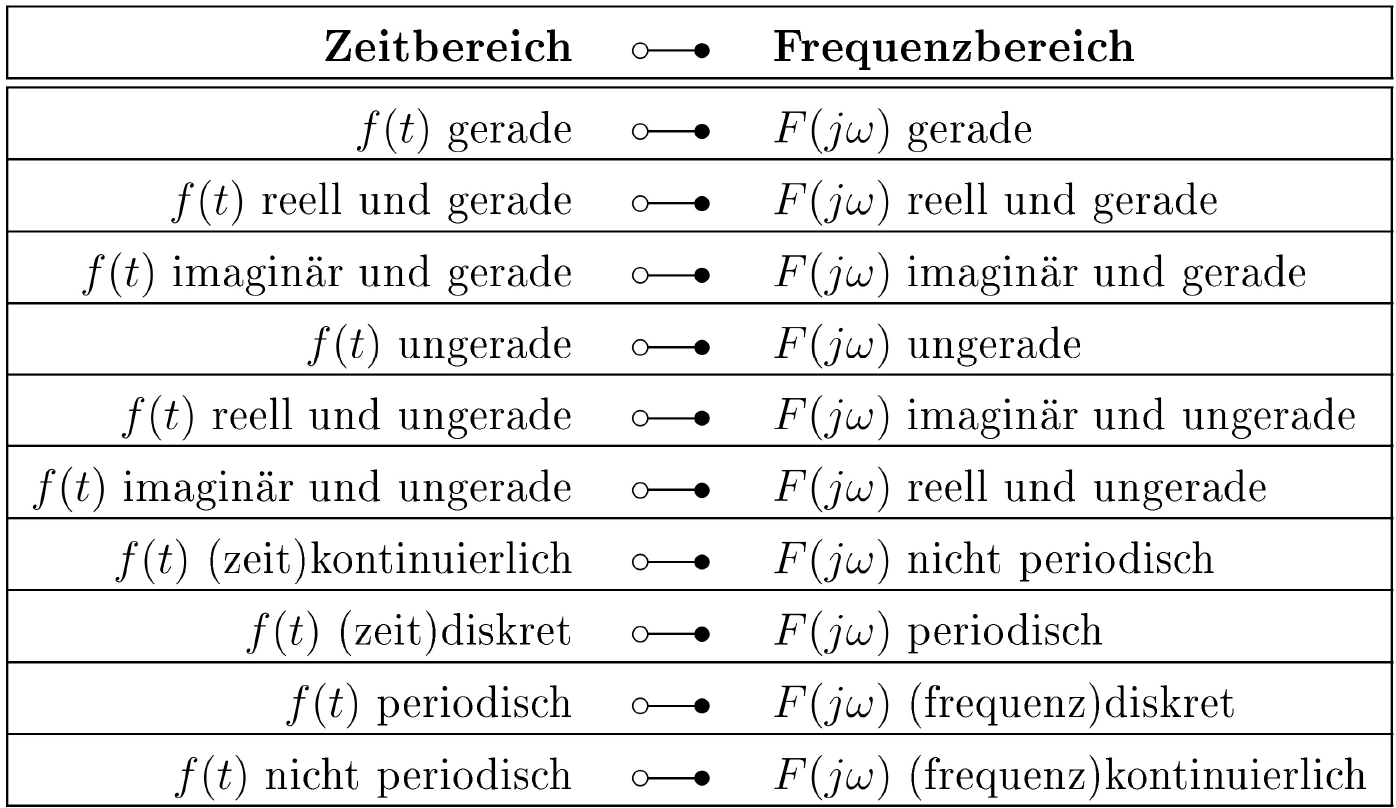
\includegraphics[width=\columnwidth]{images/eigenschaften_fourier_transformation}

\begin{center}
	\begin{tabular}{l c l}
		$f(t)$ reell 		& $\laplace$ 	& $F(-\jimg \omega) = F^*(\jimg \omega)$ konjugiert komplex	\\
		$f(-t) = f^*(t)$ 	& $\laplace$ 	& $F(\jimg \omega)$ reell
	\end{tabular}
\end{center}


\subsubsection{Linearität}

\vspace{-0.2cm}
$$ \boxed{ \alpha \cdot f(t) + \beta \cdot g(t) \, \laplace \, \alpha \cdot F(\jimg \omega) + \beta \cdot G(\jimg \omega)  \quad (\alpha, \, \beta \in \mathbb{C}) } $$


\subsubsection{Parseval's Theorem}

\vspace{-0.2cm}
$$ \boxed{ \int\limits_{- \infty}^{\infty} f(t) \, g^*(t) \, \diff t \, \laplace \, \frac{1}{2 \pi} \int\limits_{- \infty}^{\infty} F(\jimg \omega) \, G^*(\jimg \omega) \, \diff \omega } $$


\subsubsection{Bessel's Theorem (Rayleigh's Theorem)}

\vspace{-0.2cm}
$$ \boxed{ \int\limits_{- \infty}^{\infty} | f(t) | ^2 dt \, \laplace \, \frac{1}{2  \pi} \int\limits_{- \infty}^{\infty}  | F(\jimg \omega) |^2 \, \diff \omega } $$



\subsubsection{Ähnlichkeit (Streckung)}

\vspace{-0.2cm}
$$ \boxed{ f(\alpha \, t) \, \laplace \, \frac{1}{| \alpha |} F \Big( \jimg \, \frac{\omega}{\alpha} \Big) \quad \alpha \in \mathbb{R} \setminus \{ 0 \} } $$


\subsubsection{Verschiebung im Zeitbereich}

\vspace{-0.2cm}
$$ \boxed{ f( t \pm t_0 ) \, \laplace \, F(\jimg \omega) \, e^{\pm \jimg \omega t_0} } $$


\subsubsection{Verschiebung im Frequenzbereich}

\vspace{-0.2cm}
$$ \boxed{ f( t ) \, e^{\pm \jimg \omega_0 t} \, \laplace \, F(\jimg ( \omega \mp \omega_0 )) } $$


\subsubsection{Ableitung im Zeitbereich}

\vspace{-0.2cm}
$$ \boxed{ \frac{d^n f(t)}{d t^n}  \, \laplace \, (\jimg \omega)^n \, F(\jimg \omega) \quad n \in \mathbb{N}_0} $$


\subsubsection{Ableitung im Frequenzbereich}

\vspace{-0.2cm}
$$ \boxed{ t^n f(t) \, \laplace \, \jimg^n \frac{d F(\jimg \omega)}{d \omega^n} \quad n \in \mathbb{N}_0} $$


\subsubsection{Faltung im Zeitbereich (Multiplikation im Frequenzbereich)}

\vspace{-0.2cm}
$$ \boxed{ f(t)  * g(t) = \int\limits_{-\infty}^{\infty} f(\tau) \, g(t - \tau) \, d \tau \, \laplace \, F(\jimg \omega) \cdot G(\jimg \omega)  } $$


\subsubsection{Faltung im Frequenzbereich (Multiplikation im Zeitbereich)}

\vspace{-0.2cm}
$$ \boxed{ f(t) \cdot g(t) \, \laplace \, \frac{1}{2 \pi} F(\jimg \omega) * G(\jimg \omega) } $$

\subsubsection{Vertauschungssatz (Dualität)}

\vspace{0.2cm}

\begin{minipage}[c]{0.48\columnwidth}
	$$ \boxed{ f(t) \, \laplace \, F(\jimg \omega) } $$
\end{minipage}
\hfill
\begin{minipage}[c]{0.48\columnwidth}
	$$ \boxed{ F(t) \, \laplace \, 2 \pi \cdot f(- \jimg \omega) } $$
\end{minipage}


\subsubsection{Modulation}

\vspace{-0.2cm}
$$ \boxed{ \cos(\alpha t) \cdot f(t) \, \laplace \, \frac{1}{2} \cdot\Big[ F(\jimg ( \omega - \alpha)) + F(\jimg(\omega + \alpha)) \Big] } $$
$$ \boxed{ \sin(\alpha t) \cdot f(t) \, \laplace \, \frac{1}{2 \jimg} \cdot\Big[ F(\jimg ( \omega - \alpha)) - F(\jimg(\omega + \alpha)) \Big] } $$


\subsubsection{Zeitumkehrunng}

\vspace{-0.2cm}
$$ \boxed{ f(-t) \, \laplace \, F(-\jimg \omega) } $$


\subsubsection{Integration im Zeitbereich}

\vspace{-0.2cm}
$$ \boxed{ \int\limits_{-\infty}^t  f(\tau) \, d \tau \, \laplace \, \frac{F(\jimg \omega)}{\jimg \omega} + F(\jimg0) \pi \delta(\omega) } $$


\subsubsection{Anfangswerte}

\vspace{-0.2cm}
$$ \boxed{ f(0) = \frac{1}{2 \pi}  \int\limits_{-\infty}^{\infty}  F(\jimg \omega) \, \diff \omega \qquad \qquad F(\jimg0) = \int\limits_{-\infty}^{\infty} f(t) \, \diff t } $$


\subsubsection{Unendlich lange Folge von Dirac-Pulsen}

\vspace{-0.2cm}
$$ \boxed{ \sum\limits_{n = -\infty}^{\infty}  \delta(t - n \cdot t_0) \, \laplace \,   \sum\limits_{n = -\infty}^{\infty} \frac{2 \pi}{t_0}  \Big( \omega - n \cdot \frac{2 \pi}{t_0} \Big)  } $$


\subsection{AKF und Leisutngsdichtespektrum}{132}

\subsubsection{Leistungsdichtespektrum}

Die \textbf{normierte Leistung $\bm{P_n}$} eines \textbf{Leistungssignals $\bm{f(t)}$} kann mit der Hilfe des 
\textbf{Leistungsichtespektrums $\bm{\Phi(\jimg \omega)}$} beschrieben werden.
$$ \boxed{  P_n = \lim\limits_{T \to \infty} \frac{1}{T} \int\limits_{-T/2}^{T/2} | f(t) |^2 \, \diff t
	= \frac{1}{2 \pi} \int\limits_{-\infty}^{\infty} \Big( \lim\limits_{T \to \infty} \frac{|F(\jimg \omega)|^2}{T} \Big) \, \diff \omega } $$

\vspace{0.2cm}

Der Integrand wird als \textbf{Leistungsichtespektrums $\bm{\Phi(\jimg \omega)}$} bezeichnet:
$$ \boxed{ \Phi(\jimg \omega) = \lim\limits_{T \to \infty} \frac{|F(\jimg \omega) |^2}{T} } $$

\vspace{0.2cm}

Die \textbf{normierte Leisung $\bm{P_n}$} ist somit:
$$ \boxed{ X^2 = \varphi_{xx}(0) = P_n = \frac{1}{2 \pi}  \int\limits_{- \infty}^{\infty}  \Phi(\jimg \omega) \, \diff \omega } $$


\subsubsection{Energiedichtespektrum}
Analog zum Leistungsdichtespektrum lässt sich für ein \textbf{Energiesignal} (Klasse 1) das 
\textbf{Energiedichtespektrum $\bm{E(\jimg \omega)}$} finden
$$ \boxed{ W_n = \lim\limits_{T \to \infty} \int\limits_{-T/2}^{T/2} |f(t)|^2 \, \diff t = \frac{1}{2 \pi}  \int\limits_{- \infty}^{\infty} |F(\jimg \omega)|^2 \, d\omega } $$

\vspace{0.2cm}

Das \textbf{Energiedichtespektrum $\bm{E(\jimg \omega)}$} ist somit
$$ \boxed{ E(\jimg \omega) = |F(\jimg \omega)|^2 } $$


\subsection{Wiener-Chintschin Theorem}{133}

\subsubsection{Aperiodische Leistungssignale (Klasse 2b)}

Die AKF und das Leistungsdichtespektrum sind ein Fourier-Transformationspaar
$$ \boxed{ \varphi_{xx}(t) = \frac{1}{2 \pi} \int\limits_{- \infty}^{\infty} \Phi(\jimg \omega) \, e^{\jimg \omega t} \, d\omega \, \laplace \, \Phi(\jimg \omega) 
	= \int\limits_{- \infty}^{\infty} \varphi_{xx}(t) \, e^{-\jimg \omega t} \, \diff t } $$


\subsubsection{Periodische Leistungssignale (Klasse 2a) }

$$ \boxed{ \varphi_{xx}(t) = \sum\limits_{k = - \infty}^{\infty} |c_k|^2  \, e^{\jimg \frac{2 \pi k}{T_0} t } \, \laplace \, \Phi(\jimg \omega) 
	= \sum\limits_{k = - \infty}^{\infty}  |c_k|^2 \delta \Big( \omega - \frac{2 \pi k}{T_0} \Big) } $$


\subsubsection{Energiesignale (Klasse 1) }
Die AKF und das Energiedichtespektrum sind ein Fourier-Transformationspaar
$$ \boxed{ \varphi_{xx}(t) = \frac{1}{2 \pi} \int\limits_{- \infty}^{\infty} E(\jimg \omega) \, e^{\jimg \omega t} \, d\omega \, \laplace \, E(\jimg \omega)
	= \int\limits_{- \infty}^{\infty} \varphi_{xx}(t) \, e^{-\jimg \omega t} \, \diff t } $$

\columnbreak

